\subsection{Overview}

The syntax has been designed %to use as few XML elements as possible and to rely on XML attributes to setup the element behavior in a particular context.
as a restricted but still complete set of XML elements. It relies on XML attributes to setup the element behavior in a particular context.
As shown in table \ref{tbl:syntax-ele} the mapping elements  are used %can be grouped 
in three different scopes. There are only three elements for the models structure itself. We assume that any data hierarchy  can be represented by a combination of collections  \texttt{COLLECTION}, tuples  \texttt{INSTANCE}, and simple values  \texttt{ATTRIBUTE}. The other elements are either to set the mapping block structure or to connect data to each other.

\begin{table}[!htbp]
\small
\centering
\begin{tabulary}{\linewidth}{|c|J|}       
       \hline 
            \textbf{Scope} & 
            \textbf {Elements}\\
       \hline         
       \hline  
             Data modeling tags & 
             \texttt{ATTRIBUTE} \texttt{INSTANCE} \texttt{COLLECTION} \\
       \hline  
             Mapping block structure & 
             \texttt{VODML} \texttt{MODEL} \texttt{REPORT} \texttt{TEMPLATES} \texttt{GLOBALS} \\
       \hline  
             Data references and identification & 
             \texttt{REFERENCE} \texttt{JOIN}  \texttt{FOREIGN\_KEY} \texttt{PRIMARY\_KEY} \texttt{WHERE} \\
       \hline
     \end{tabulary}
     \caption{Mapping elements grouped by scopes.} 
     \label{tbl:syntax-ele}
\end{table}


As shown in Table \ref{tbl:syntax-att} and following the \texttt{VODML} pattern, any model node is characterized by a role  \texttt{@dmrole}  and a type  \texttt{@dmtype}.  All of the other attributes are used to bind data with either VOTable elements or other mapping elements.
 
\begin{table}[!htbp]
\small
\centering
\begin{tabulary}{\linewidth}{|c|J|}       
       \hline 
            \textbf{Scope} & 
            \textbf {Attributes}\\
       \hline         
       \hline  
             Model related & 
             \texttt{@name} \texttt{@url} \\
       \hline  
             Modeled node related & 
             \texttt{@dmrole} \texttt{@dmtype} \\
       \hline  
             Related to attribute values & 
             \texttt{@value} \texttt{@unit} \texttt{@arrayindex} \\
       \hline  
             Related to VOTable elements & 
             \texttt{@tableref} \texttt{@ref} \\
       \hline  
             Mapping element identification& 
             \texttt{@dmref} \texttt{@dmid} \texttt{@sourceref} \texttt{@primarykey} \texttt{@foreignkey} \\
       \hline
     \end{tabulary}
     \caption{Attributes of mapping elements grouped by scopes.} 
     \label{tbl:syntax-att}
 \end{table}
 
 


  \begin{figure}[h]
    \begin{center}
      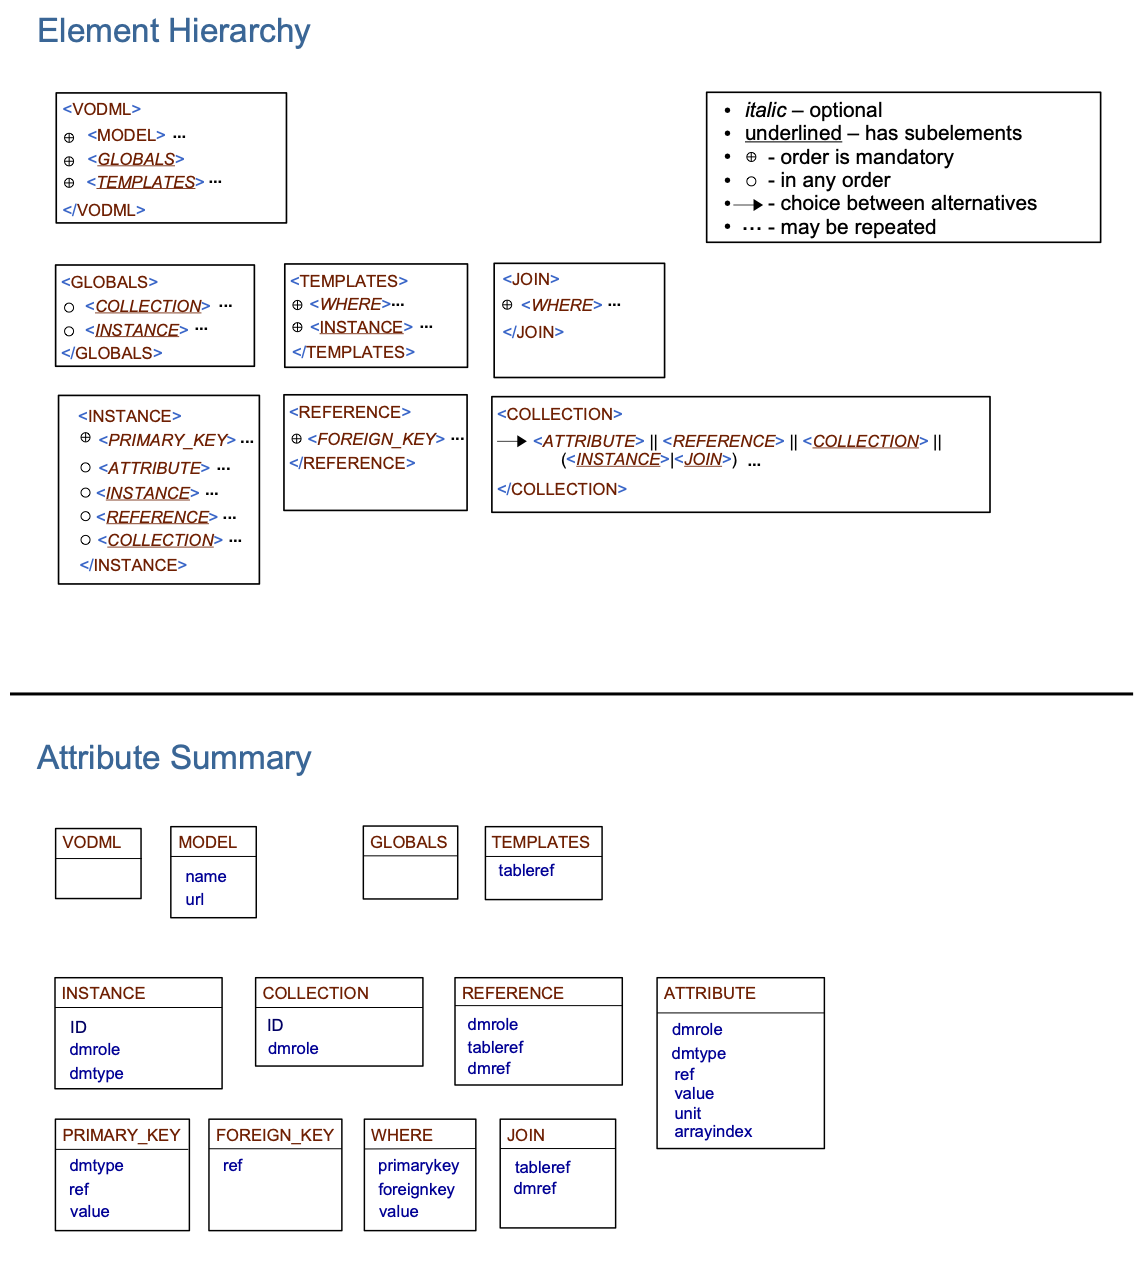
\includegraphics[width=1.2\textwidth]{mivot-summary.png}
      \caption{Annotation Syntax Summary.}
      \label{fig:summary}
    \end{center}
  \end{figure}


\subsection{Reader's Guide}

Each element subsection come with 2 or 3 tables: 1) one giving the role of each attribute, 
2) one giving the allowed children elements (when relevant), 3) one telling when each attribute 
is mandatory (MAND), optional (OPT) or prohibited (NO). 
The content of these tables is a transcription of the XSD assertions.

In the following normative subsections, all mapping patterns are illustrated with XML snippets.
Most of these excerpts are taken out of a complete VOTable listed in appendix \ref{appendix_A}.
The others are out of the box, they refer to model elements or VOTable metadata that do not exist 
but that have been chosen to achieve better readability. 
Readers can have a look at \url{https://github.com/ivoa-std/ModelInstanceInVot/tree/master/data-sample} 
to inspect most of them in a context of real data.

